\documentclass[a4paper]{article}

\usepackage[english]{babel}
\usepackage[utf8]{inputenc}
\usepackage{fullpage}
\usepackage{amsmath}
\usepackage{graphicx}
\usepackage[colorinlistoftodos]{todonotes}
\usepackage{hyperref}
\usepackage{amssymb}
\usepackage{outline} \usepackage{pmgraph} \usepackage[normalem]{ulem}
\usepackage{graphicx} \usepackage{verbatim}
\usepackage{amssymb} %checklist

\usepackage{wasysym} %checkedbox
\definecolor{mypink1}{rgb}{0.858, 0.188, 0.478}
\definecolor{mypink2}{RGB}{219, 48, 122}
\definecolor{mypink3}{cmyk}{0, 0.7808, 0.4429, 0.1412}
\definecolor{mygray}{gray}{0.4}
 

%\usepackage[dvipsnames]{xcolor} 

% \usepackage{minted} % need `-shell-escape' argument for local compile

\title{
    \vspace*{1in}
    
\includegraphics[width=3.95in]{figures/uff-logo.png} \\
    \vspace*{1.2in}
    \textbf{\huge Weekly Report Master Thesis}
    \vspace{0.2in}\\
    \vspace{0.2in}
}

\author{Luigy Machaca \\
    %\vspace*{0.5in} \\
    \textbf{luigyarcana@id.uff.br} \\
    % \vspace*{1in}
}

\date{\today}


\begin{document}

\maketitle
\setcounter{page}{0}
\thispagestyle{empty}
\newpage


\section{Research Project}
In this project, we are going to developing an object detection and tracking system using modern computer vision technology. The project delivers and implemented a tracking system. It consists of a hybrid of online and offline tracking algorithm is applicable to areas such as object tracking surveillance videos or semi-autonomous cameras technology\cite{re3}. It is applicable to areas as a stand-alone camera system or one that could easily be embedded into an even larger system. This report expressed how has been to development since April.

\section{ Background Research  }

Research and reading carried out as the background research related to the project are described. We will outline key themes that the platform where runs and described the general computer vision techniques included.

\subsection{Docker}
%\subsection{\textcolor{mygray}{Docker}}
%\iffalse
Docker is a tool designed to make it easier to create, deploy, and run applications by using containers. Containers allow a developer to package up an application with all of the parts it needs, such as libraries and other dependencies, and ship it all out as one package. See Figure \ref{fig:docker} 


\begin{figure}[hb]
    \centering
    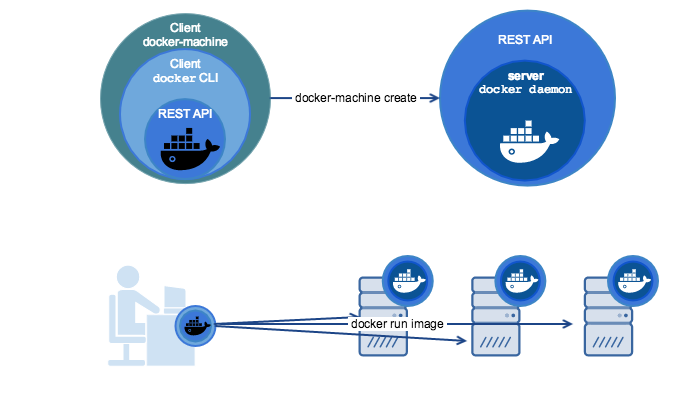
\includegraphics[width=0.5\textwidth]{figures/docker.png}
    \caption{The Docker daemon is a service that runs on your host operating system. It currently only runs on Linux because it depends on a number of Linux kernel features, but there are a few ways to run Docker on MacOS and Windows too. TheDocker daemon itself exposes a REST API.}
    \label{fig:docker}
\end{figure}
%\fi


\subsection{Nvidia \& Docker}
%\subsection{\textcolor{mygray}{Nvidia \& Docker}}
%\iffalse
NVIDIA uses containers to develop, test, benchmark, and deploy deep learning (DL) frameworks and HPC applications. We have use building and deploying GPU containers at scale using NVIDIA-Docker.  A variety of customers used NVIDIA-Docker to containerize and run GPU accelerated workloads. See Figure \ref{fig:nvidia-docker}

\begin{figure}[hb]
    \centering
    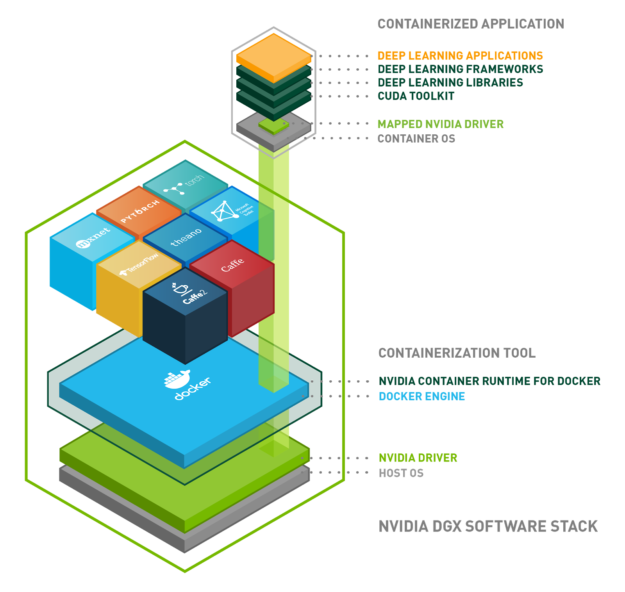
\includegraphics[width=0.4\textwidth]{figures/nvidia-docker.png}
    \caption{As a result, the redesigned NVIDIA-Docker moved the core runtime support for GPUs into a  library called libnvidia-container. The library relies on Linux kernel primitives and is agnostic relative to the higher container runtime layers. This allows easy extension of GPU support into different container runtimes such as Docker.}
    \label{fig:nvidia-docker}
\end{figure}
%\fi 


\subsection{Algorithm}
%\subsection{\textcolor{mygray}{Algorithm}}
\subsubsection{Re3: Real-Time Recurrent Regression Networks for Visual Tracking of Generic Objects.}
%\subsubsection{\textcolor{mygray}{Re3: Real-Time Recurrent Regression Networks for Visual Tracking of Generic Objects.}

%\iffalse
The tracking pipeline, consists of:
\begin{itemize}
    \item convolutional layers to embed the object appearance, 
    \item recurrent layers to remember appearance and motion information, 
    \item and a regression layer to output the location for the object. 
\end{itemize}
See Figure \ref{fig:re3}

\begin{figure}[hb]
    \centering
    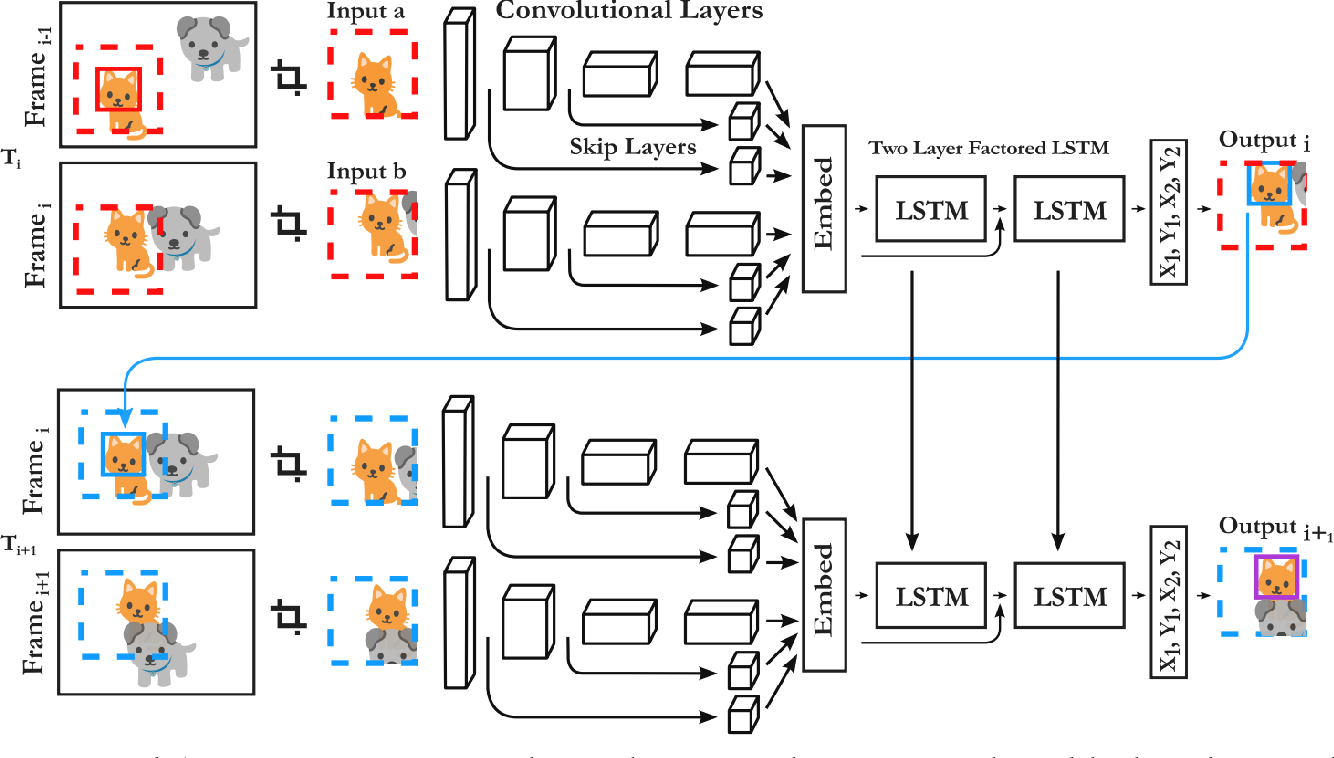
\includegraphics[width=0.6\textwidth]{figures/pipeline-re3.png}
    \caption{
            cccccccccc
    }
    \label{fig:re3}
    \medskip
    \small 
        \begin{itemize}
        \item Image crop pairs are fed in at each time step.
        \item Both crops are centered around the object\'s location in the previous frame 
        \item and padded to two times the width and height of the object. 
        \item before every pooling state, to add a skip layer to preserve high-resolution spatial information.
        \item The weights from the two image streams are shared.
        \item The output from the convolutional layers feeds into a single fully connected layer and  and LSTM.
        \item The network predicts the top left and bottom right corners if the new bounding box.  
        \end{itemize}
\end{figure}
%%\fi


%\subsection{\textcolor{mygray}{Dataset}}
\subsection{Dataset}

%\iffalse
The VOT challenges provide the visual tracking community with a precisely defined and repeatable way of comparing short-term trackers as well as a common platform for discussing the evaluation and advancements made in the field of visual tracking.
\cite{VOT2014} \cite{VOT2016}
\begin{itemize}
    \item VOT 2014
    \item VOT 2016
\end{itemize}
%\fi



%\iffalse
%\subsection{Doxygen}
%Doxygen is a tool for documenting code that is compatible with Python. Doxygen provides most of the functions, but it is also a bit complicated. Because of the amount of work he does, he does it at a very fast speed.
%\begin{itemize}
%    \item Written and compiled in C ++, this is the fastest of the tools by far.
%    \item You can generate documentation in several ways, not just in HTML.
%    \item Supports Markdown and documentation pages
%    \item You can easily see the source directly from the documentation.
%    \item Diagrams with the structure of your code. 
%\end{itemize}
%\fi

\subsection{Opencv-python}
OpenCV (Open Source Computer Vision Library) is an open source computer vision and machine learning software library. OpenCV was built to provide a common infrastructure for computer vision applications and to accelerate the use of machine perception in the commercial products. Being a BSD-licensed product, OpenCV makes it easy for businesses to utilize and modify the code.

\begin{itemize}
    \item Often, we have to capture live stream with camera. OpenCV provides a very simple interface to this. 
    \item we are using the in-built webcam of my laptop
    \item Let’s capture a video from the camera, and split video frame per frame. 
\end{itemize}



\section{Progress}



%\iffalse
%\begin{description}
%\item [$\checkmark$ \textcolor{mygray}{Step 1}] Research, install and test Docker \& Nvidia on remote PC.} 
%\item[$\checkmark$ \textcolor{mygray}{Step 2}] \textcolor{mygray}{ Building instances for Nvidia-docker.}
%\item[$\checkmark$ \textcolor{mygray}{Step 3}] \textcolor{mygray}{Fixed problems for network connection and port of remote PC  with a VPN.}
%\item[$\checkmark$ \textcolor{mygray}{Step 4}] \textcolor{mygray}{Replicate results and test of Re3 \cite{re3} on Docker container.}
%\item[$\checkmark$ \textcolor{mygray}{Step 5}] \textcolor{mygray}{Fixed problems with CUDA version and requirements of Re3.}
%\item[$\checkmark$ Step 6] \textbf{Analyzing} Copacabana surveillance videos.
%\item[$\checkmark$ Step 7] Copacabana videos has been \textbf{spitting} frame per frame. [opencv-python]
%\item[$\checkmark$ Step 8] The code re3 is being \textbf{documented}. [Doxygen]
%\end{description}
%\fi

\begin{description}
\item [$\checkmark$ Step 1] Research, install and test Docker \& Nvidia on remote PC.
\item[$\checkmark$ Step 2] Building instances for Nvidia-docker.
\item[$\checkmark$ Step 3] Fixed problems for network connection and port of remote PC  with a VPN.
\item[$\checkmark$ Step 4] Replicate results and test of Re3 \cite{re3} on Docker container.
\item[$\checkmark$ Step 5] Fixed problems with CUDA version and requirements of Re3.
\item[$\checkmark$ Step 6] \textbf{Analyzing} Copacabana surveillance videos.
\item[$\checkmark$ Step 7] Copacabana videos has been \textbf{spitting} frame per frame. [opencv-python]
%\item[$\checkmark$ Step 8] The code re3 is being \textbf{documented}. [Doxygen]
\item[$\square$ Step 8] \textbf{Testing} Re3 with multiple people.
\item[$\square$ Step 10] Create a \textbf{Pipeline}, where Re3 is going to be a module of \textit{Framework}.
%\item[$\square$ Step 11] \textbf{Training} with data set.
 


\section{Plan}

\begin{tabular}{rl}
	\textbf{Objective:} & Framework tracking multiple people \\
    %\textbf{Deadline:} & 22 may 
\end{tabular}


\begin{description}
    %\item[\normalfont 2019.02.07---2019.05.14] Do something.
    %\item[\normalfont 2019.05.15---2019.05.22] Do something else.
    %\item[\normalfont 2019.05.23---2019.05.31] Do a lot lot lot lot lot lot lot lot lot lot lot lot of things.
    \item[$\square$ Step 11] move all project to NIXos
    \item[$\square$ Step 12] improve module \textbf{tracking}, where algorithm      \textbf{YOLO} is going to be a sub-module of \textit{tracking}.
    \item[$\square$ Step 13]  

\end{description}


% If you don't cite any references, please comment the following two lines
\nocite{*}
\bibliographystyle{ieee}
\bibliography{ref.bib}

\end{document}

